\documentclass[11pt,a4paper]{article}
\usepackage[margin=2.2cm]{geometry}
\usepackage[utf8]{inputenc}
\usepackage[T1]{fontenc}

\usepackage{graphicx}
\usepackage{amsmath}
\usepackage{booktabs}
\usepackage{array}
\usepackage{tabularx}
\usepackage{xcolor}
\usepackage{tikz}
\usetikzlibrary{arrows.meta,positioning,shapes.geometric,fit,backgrounds}
\usepackage{hyperref}
\usepackage{caption}
\usepackage{subcaption}
\usepackage{enumitem}
\usepackage{float}
\hypersetup{colorlinks=true, linkcolor=blue!50!black, urlcolor=blue!50!black, citecolor=blue!50!black}
\setlist{nosep}
\captionsetup{font=small, labelfont=bf}
\graphicspath{{figures/}}
\newcommand{\code}[1]{\texttt{\small #1}}

\title{\textbf{FallVision: Person Collapse Detection in Video}\\[4pt]
\large DS5602 Computer Vision --- Course Project Report}
\author{\small Team ID, member names and roll numbers: \texttt{TEAM.md} in the submission package\\
\small (Member 1, Member 2, Member 3 as referred to in Section~9)}
\date{November 2026}

\begin{document}
\maketitle

\begin{abstract}
We built a system that detects when a person falls (collapses) in a video and reports \emph{who} (track ID),
\emph{where} (bounding box) and \emph{when} (decision time, with the estimated onset recorded separately),
processing the video frame by frame using only current and past frames. The method combines a pretrained
YOLO11m-pose model and ByteTrack with 92 normalised skeleton features per frame and a small GRU classifier
trained by us on 2-second windows labelled \emph{normal / falling / fallen} with the OmniFall annotations of
five public datasets. Every modelling choice (model, score, threshold, decision lag) was made on a validation
split; the test sets were evaluated once. The submitted system reaches a video-level F1 of 0.875 on GMDCSA24
(unseen subjects), 0.968 on staged Le2i/CAUCAFall clips, 0.855 on 818 real-world OOPS clips, and catches 15 of
20 of our own recordings with no false alarm. This report describes the task, the data, every approach we tried,
the training (with learning curves), the results, the failure cases and how to reproduce the work.
\end{abstract}

\section{Problem statement}
The input is a video; the output is a sequence of per-frame predictions and alarms of label
\code{person\_collapse}. The system has to work on video it has never seen, indoors and at night, with one
or several people, and it must raise an alarm only for a real collapse. Table~\ref{tab:req} lists the design
goals we set at the start and how the final system meets them.

\begin{table}[H]\centering\small
\begin{tabularx}{\textwidth}{@{}>{\raggedright\arraybackslash}p{4.6cm}X@{}}\toprule
\textbf{Design goal} & \textbf{How it is met} \\ \midrule
A single pretrained vision model (YOLO11) & YOLO11m-pose finds people and 17 joints; nothing else is pretrained (ByteTrack has no learned weights). \\
Falls from sitting must be caught & Falls from chairs and beds are in the training data; window labels come from the fall \emph{movement}, not from standing height. \\
No false alarms (lying down, sitting fast, exercise are not falls) & Those activities are labelled \emph{normal} and weighted $\times 3$ as hard negatives; the threshold is chosen for best validation F1, ties broken by fewer false alarms. \\
Must work at night & Skeleton features instead of pixels; ``night'' augmentation (joints hidden, confidences lowered). \\
Tested on unseen videos & Official cross-subject splits; OOPS and our own recordings were never used for any choice. \\
Causal, real-time operation: past frames only, alarms as they occur, state reset per video & The causal engine \code{src/fv\_engine.py} used by \code{infer.py}; \code{decision\_timestamp\_s} = latest frame used, \code{onset\_estimate\_s} recorded separately. \\
One configuration file, offline inference, a single command, machine-readable outputs & \code{infer.py --source --config --output-dir --device --no-display} writes \code{predictions.jsonl}, \code{alarms.jsonl}, \code{run\_summary.json}; weights are in the package; \code{YOLO\_OFFLINE=1}. \\
\bottomrule\end{tabularx}
\caption{Design goals and where they are met.}\label{tab:req}
\end{table}

\section{Data, labels and splits}
\begin{table}[H]\centering\small
\begin{tabularx}{\textwidth}{@{}lrXll@{}}\toprule
\textbf{Dataset} & \textbf{Videos} & \textbf{Content} & \textbf{Role} & \textbf{Licence}\\ \midrule
GMDCSA24 & 160 & staged falls and daily activities, 4 subjects, home & train S1 / val S2 / \textbf{test S3--4} & MIT\\
Le2i & 190 & staged falls, home / office / lecture room & train / val / test (official) & research\\
CAUCAFall & 97 & staged falls, varied lighting, hard daily actions & train / val / test (official) & research\\
MCFD & 192 & staged falls, several cameras & train only & research\\
OOPS (fall clips) & 818 & real-world internet videos of people falling & \textbf{test only} & non-commercial\\
Own recordings & 20 & day / night, near / far, 1--9 people, falls from standing, walking, sitting, jumping & \textbf{test only} & private\\
\bottomrule\end{tabularx}
\caption{Datasets. Split sizes: train 426, validation 76, test\_gmdcsa24 80, test\_staged 57, test\_oops 818, test\_own 20.}
\end{table}

\textbf{Labels and splits.} OmniFall~\cite{omnifall} provides frame-accurate activity segments (16 classes:
walk, fall, fallen, sit down, sitting, lie down, lying, stand up, standing, other, kneel down, kneeling, squat down,
squatting, crawl, jump) and official cross-subject splits for all five datasets, so no actor appears in two
splits. For training, each 2-second window gets one of three classes (\code{src/make\_windows.py}):
\emph{falling} if it overlaps a fall segment by at least 0.5\,s (or half of a shorter fall), \emph{fallen} if it
ends while the person is lying after a fall, and \emph{normal} otherwise --- deliberately including lying down
on purpose, sitting down and exercise, the main sources of false alarms. Windows whose OmniFall class at the end
is sit down, lie down, lying, other, kneel/squat, crawl or jump are the \emph{hard negatives}. Window counts:
12\,587 training (9\,683 normal, 1\,795 falling, 1\,109 fallen) and 1\,262 validation windows.
Figure~\ref{fig:fall} shows a labelled fall from GMDCSA24.

\begin{figure}[H]\centering
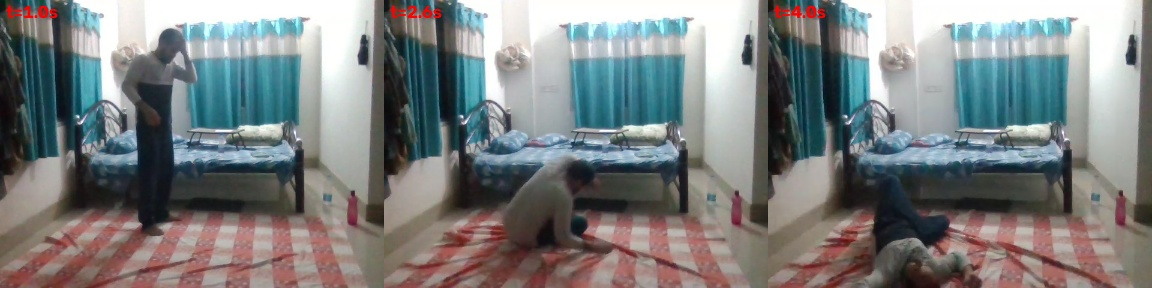
\includegraphics[width=\textwidth]{fall_sequence.jpg}
\caption{A GMDCSA24 fall at $t=1.0$, $2.4$ and $4.0$\,s: standing, the fall movement (\emph{falling}), lying after the fall (\emph{fallen}).}\label{fig:fall}
\end{figure}

\section{The pipeline}
Figure~\ref{fig:pipeline} shows the complete system; every stage is one script in \code{src/} and
\code{run\_pipeline.py} runs them in order on CPU or GPU (the Kaggle notebooks call the same scripts).

\begin{figure}[H]\centering
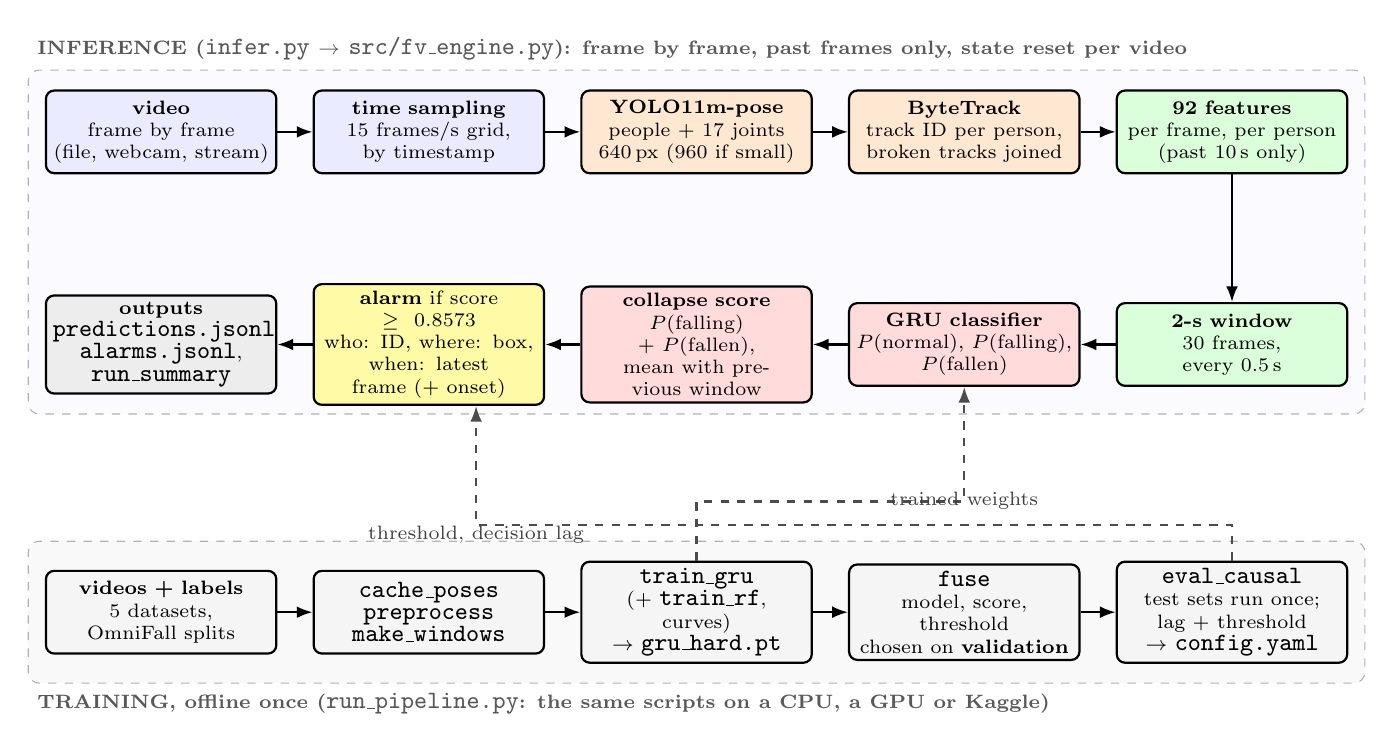
\begin{tikzpicture}[font=\scriptsize, >={Latex[length=2mm]}, x=1cm, y=1cm,
  st/.style={draw, rounded corners=3pt, align=center, text width=2.75cm, minimum height=1.05cm, inner sep=2.5pt, thick, fill=#1},
  lane/.style={draw=gray!60, dashed, rounded corners=4pt, inner xsep=6pt, inner ysep=7pt},
  lab/.style={font=\scriptsize\bfseries\color{gray!70!black}}]
% ---- row 1: inference, per frame ----
\node[st=blue!8]   (v)  at (0,0)    {\textbf{video}\\frame by frame\\(file, webcam, stream)};
\node[st=blue!8]   (s)  at (3.4,0)  {\textbf{time sampling}\\15 frames/s grid,\\by timestamp};
\node[st=orange!18](p)  at (6.8,0)  {\textbf{YOLO11m-pose}\\people + 17 joints\\640\,px (960 if small)};
\node[st=orange!18](t)  at (10.2,0) {\textbf{ByteTrack}\\track ID per person,\\broken tracks joined};
\node[st=green!14] (f)  at (13.6,0) {\textbf{92 features}\\per frame, per person\\(past 10\,s only)};
% ---- row 2: decision, per person ----
\node[st=green!14] (w)  at (13.6,-2.7) {\textbf{2-s window}\\30 frames,\\every 0.5\,s};
\node[st=red!14]   (g)  at (10.2,-2.7) {\textbf{GRU classifier}\\$P$(normal), $P$(falling),\\$P$(fallen)};
\node[st=red!14]   (sc) at (6.8,-2.7)  {\textbf{collapse score}\\$P$(falling) $+$ $P$(fallen),\\mean with previous window};
\node[st=yellow!35](al) at (3.4,-2.7)  {\textbf{alarm} if score $\ge 0.8573$\\who: ID, where: box,\\when: latest frame (+ onset)};
\node[st=gray!14]  (o)  at (0,-2.7)    {\textbf{outputs}\\\code{predictions.jsonl}\\\code{alarms.jsonl}, \code{run\_summary}};
\draw[->, thick] (v)--(s); \draw[->, thick] (s)--(p); \draw[->, thick] (p)--(t); \draw[->, thick] (t)--(f);
\draw[->, thick] (f)--(w);
\draw[->, thick] (w)--(g); \draw[->, thick] (g)--(sc); \draw[->, thick] (sc)--(al); \draw[->, thick] (al)--(o);
% ---- row 3: training, offline ----
\node[st=gray!8] (d)  at (0,-6.1)    {\textbf{videos + labels}\\5 datasets,\\OmniFall splits};
\node[st=gray!8] (c1) at (3.4,-6.1)  {\code{cache\_poses}\\\code{preprocess}\\\code{make\_windows}};
\node[st=gray!8] (c2) at (6.8,-6.1)  {\code{train\_gru}\\(+ \code{train\_rf}, curves)\\$\rightarrow$ \code{gru\_hard.pt}};
\node[st=gray!8] (c3) at (10.2,-6.1) {\code{fuse}\\model, score, threshold\\chosen on \textbf{validation}};
\node[st=gray!8] (c4) at (13.6,-6.1) {\code{eval\_causal}\\test sets run once;\\lag + threshold $\rightarrow$ \code{config.yaml}};
\draw[->, thick] (d)--(c1); \draw[->, thick] (c1)--(c2); \draw[->, thick] (c2)--(c3); \draw[->, thick] (c3)--(c4);
% dashed links training -> inference
\draw[->, thick, dashed, gray!60!black] (c2.north) -- ++(0,0.75) -| (g.south)
      node[pos=0.6, below=1pt, font=\scriptsize, gray!50!black] {trained weights};
\draw[->, thick, dashed, gray!60!black] (c4.north) -- ++(0,0.45) -| ([xshift=6mm]al.south)
      node[pos=0.55, below=1pt, font=\scriptsize, gray!50!black] {threshold, decision lag};
% ---- lanes ----
\begin{scope}[on background layer]
\node[lane, fit=(v)(f)(o)(w), fill=blue!2] (l1) {};
\node[lane, fit=(d)(c4), fill=gray!5] (l3) {};
\end{scope}
\node[lab, anchor=south west] at (l1.north west) {INFERENCE (\code{infer.py} $\rightarrow$ \code{src/fv\_engine.py}): frame by frame, past frames only, state reset per video};
\node[lab, anchor=north west] at (l3.south west) {TRAINING, offline once (\code{run\_pipeline.py}: the same scripts on a CPU, a GPU or Kaggle)};
\end{tikzpicture}
\caption{The FallVision pipeline. Top: the submitted causal system; every number shown (15\,fps, 640/960\,px, 2\,s, 0.5\,s, 10\,s, 0.8573) is read from \code{config.yaml}. Bottom: how the model and the threshold were produced; the dashed arrows are the only links between training and inference.}\label{fig:pipeline}
\end{figure}

\paragraph{Frame sampling.} A frame is processed when it lands on the next slot of a 15-per-second time grid
(by timestamp), whatever the camera's frame rate; the others are counted as skipped. The GRU was trained at
15\,fps, so timing is identical for every video.

\paragraph{Pose and tracking.} YOLO11m-pose (input 640\,px, detection confidence 0.25, people only) gives a
box, 17 COCO joints and a confidence per joint; ByteTrack assigns IDs. While the people in view are small
(standing height below 150\,px measured in a 1280-px-wide frame) the input switches to 960\,px, which the
far-camera experiments showed helps. When someone falls the tracker often gives them a new ID; a new ID that
appears within 1.5\,s and one body height of a lost one is joined to the same person
(Figure~\ref{fig:pose}, left).

\paragraph{Features (\code{src/preprocess.py}).} Per frame and person, from that person's past 10 seconds
only: 34 joint positions relative to the hip centre and divided by the standing height (90th percentile of
box height), 34 joint velocities, 17 joint confidences, and 7 whole-body cues (head-top height above the floor
and its vertical speed, box height / standing height, box aspect ratio, torso angle, hip vertical speed,
``seen'' flag). Gaps up to 0.5\,s are interpolated; longer gaps are marked as not seen. Everything is
relative, so camera distance, resolution and lighting matter less.

\paragraph{Classifier and alarm.} Every 0.5\,s the GRU reads the last 30 frames and outputs three class
probabilities. The score $P(\text{falling})+P(\text{fallen})$ is averaged with the previous window; the moment
a person's score reaches the threshold an alarm is written with the person ID, the box, the time of the
latest frame used and an onset estimate (the moment of fastest head drop in the window). The same person can
alarm again only after 10\,s below the threshold. All numbers above are in \code{config.yaml}.

\begin{figure}[H]\centering
\begin{subfigure}{0.49\textwidth}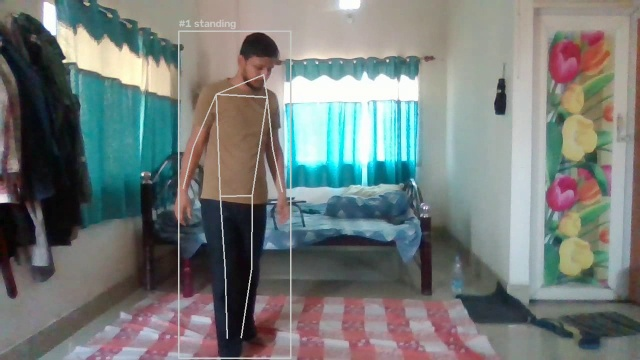
\includegraphics[width=\textwidth]{pose_frame.jpg}\caption{Pose + tracking stage: box, 17 joints, track ID.}\end{subfigure}\hfill
\begin{subfigure}{0.49\textwidth}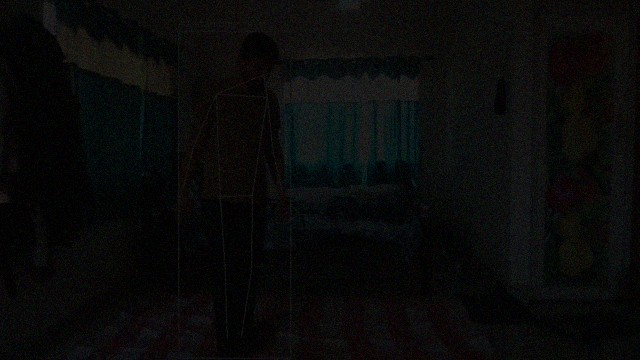
\includegraphics[width=\textwidth]{night_sim.jpg}\caption{Night simulation (darkening, gamma, noise) used in the robustness study.}\end{subfigure}
\caption{Intermediate views (GMDCSA24 frames).}\label{fig:pose}
\end{figure}

\section{Methodologies tried}
Everything below was evaluated at video level (a fall video is correct if an alarm is raised, a normal video
if none is), with precision, recall, F1, false alarms and missed falls; the numbers are in the files of
\code{results/} named in brackets.

\subsection{Rule-based baseline (\code{src/baseline\_fall.py}, \code{src/detect\_falls.py})}
YOLO11 pose + ByteTrack + a hand-written state machine per person: a fast drop of the head top, then ``down''
(box height well below the person's standing height) held for 2\,s, with a stillness check. Rules v2, tuned
on GMDCSA24 Subjects 1--2 and tested on Subjects 3--4: F1 0.870 with one false alarm (push-ups); most misses were
falls onto or from a bed or chair [\code{gmdcsa24\_*}, \code{rules\_splits.md}]. Lesson: thresholds on heights
and speeds cannot separate ``sitting down fast'' from ``falling''.

\subsection{Pose model size and input resolution}
YOLO11n-pose vs YOLO11m-pose with the same rules: F1 0.72 vs 0.87, so the medium model is used. Input 960\,px
helps far-away people (far-simulation F1 0.63 $\rightarrow$ 0.74) while 1280\,px adds false alarms
[\code{far\_*}]; final choice: 640\,px, switching to 960\,px only while people are small (resolution-independent
rule).

\subsection{Night and far-away simulations (\code{simulate\_night.py}, \code{simulate\_far.py}, \code{night\_analysis.py})}
Validation videos were darkened (gamma, noise; Figure~\ref{fig:pose}, right) and shrunk (far camera). At night
the rules' F1 fell to 0.58, through misses rather than false alarms; image brightening (CLAHE, denoising)
made it \emph{worse} (F1 0.35--0.42) and was dropped [\code{night\_*}]. The analysis showed that at night the
person is lost in 1 of 5 frames and the torso is unreadable in 1 of 3. Decision: handle it in the learned
model (night and frame-drop augmentation) rather than in the image.

\subsection{Random Forest (\code{src/train\_rf.py})}
300 trees on 460 window-summary statistics of the 92 features (class-balanced, \code{random\_state=0}). The
first learned model; it beats the rules everywhere, most on real-world video (OOPS F1 0.38 $\rightarrow$ 0.69)
[\code{rf.md}].

\subsection{GRU sequence classifier (\code{src/train\_gru.py}) --- the main model}
Input 30 frames $\times$ 92 features, standardised with the training mean and standard deviation (stored in
the model file). Two GRU layers (hidden 128, dropout 0.3), then a classifier on [last hidden state, mean of
hidden states] $\rightarrow$ 3 classes. Training: AdamW (lr $10^{-3}$, weight decay $10^{-4}$), cosine
schedule, batch 256, 40 epochs, class-weighted cross-entropy (weights $\propto 1/\sqrt{\text{count}}$),
gradient clipping 1.0, seed 0; the epoch with the best validation window macro-F1 is kept, the best checkpoint
is written whenever validation improves and the last epoch is kept with its optimizer state. Augmentation
(training only, each with probability 0.5): mirror (left/right joints swapped), rotation $\pm15^\circ$, scale
0.9--1.1, joint noise, \emph{night} (10--40\,\% of joints hidden, confidences lowered), \emph{frame drop} (up to
20\,\% of frames blank). \emph{Hard negatives $\times 3$}: normal windows of the hard classes get three times the
loss weight. Three variants were trained with the same data and seed: without augmentation, with augmentation,
and with augmentation + hard negatives (\textbf{final}, \code{gru\_hard.pt}, best epoch 16 of 40, validation
window macro-F1 0.864) [\code{gru\_noaug.md}, \code{gru.md}, \code{gru\_hard.md}].

\subsection{Model, score and threshold choice on validation (\code{src/fuse.py})}
Every model alone, the mean of every pair and of all models, two window scores
($P(\text{falling})+P(\text{fallen})$ vs $P(\text{falling})$ only) and two threshold rules (best F1;
precision $\ge 0.95$) were scored on \emph{validation only} [\code{fusion.md}]. Chosen: \code{gru\_hard} alone,
score fall+fallen, best-F1 threshold. Averaging with the Random Forest or the other GRUs did not improve
validation F1.

\subsection{Whole-video evaluation, error analysis, localization}
The complete detector was run on every test video with every person scored
(\code{eval\_system.py}); 18 failure clips were watched by hand [\code{error\_analysis.md}]; the 20 own
recordings were checked (\code{eval\_own.py}, \code{check\_own\_videos.py}). Localization was checked by eye on
36 alarm frames: the alarm box is on the person who fell in 33 (92\,\%) [\code{localization.md}].

\subsection{Hard validation set (\code{src/make\_hard\_val.py})}
To test ideas without touching the test sets, validation videos were made far away and composed into
three-person crowds (Figure~\ref{fig:hardval}). Tested and rejected: low-confidence tracking (far 18
$\rightarrow$ 17 caught, false alarms 22 $\rightarrow$ 21), fall-aware track joining (no change), and a higher
threshold (0.864, by F2 on this set), which was tested once on the test sets, lost falls and removed no false
alarms; it is disclosed in \code{results/summary.md} and was not kept [\code{system\_hv\_*},
\code{system\_final864*}].

\begin{figure}[H]\centering
\begin{subfigure}{0.62\textwidth}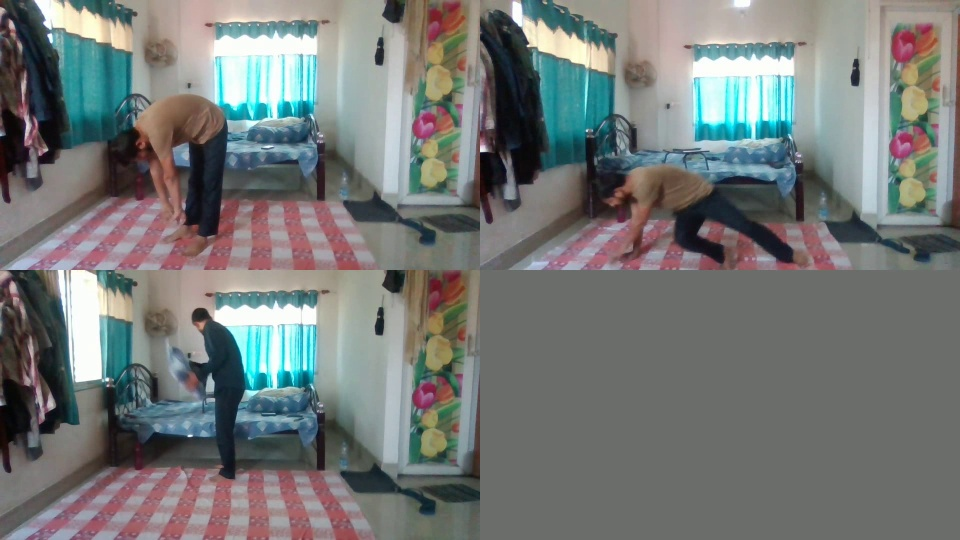
\includegraphics[width=\textwidth]{hardval_crowd.jpg}\caption{Crowd composite (three validation clips side by side).}\end{subfigure}\hfill
\begin{subfigure}{0.36\textwidth}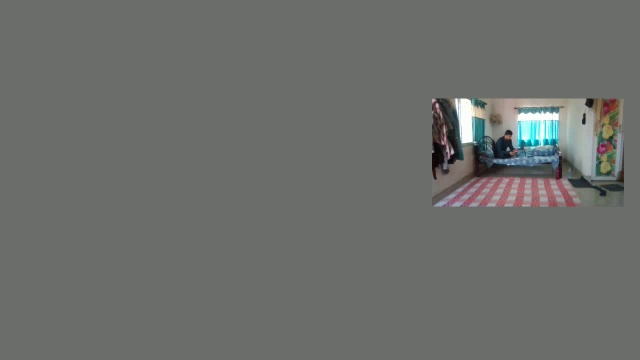
\includegraphics[width=\textwidth]{hardval_far.jpg}\caption{Far-away version of a validation clip.}\end{subfigure}
\caption{The hard validation set used for the robustness experiments.}\label{fig:hardval}
\end{figure}

\subsection{The causal engine and its evaluation (\code{src/fv\_engine.py}, \code{src/eval\_causal.py})}
Operating causally (current and past frames only) changes the features slightly (floor level and standing
height are known only from the past), so the engine used by \code{infer.py} was run on all 1\,051 validation
and test videos and the threshold was \emph{re-chosen on validation for this exact engine}: 0.8573
[\code{causal\_eval.md}]. A decision lag of 0 / 0.5 / 1.0 / 1.5\,s (score the window ending a little before the
newest frame, still past frames only) was compared by validation average precision: 0.958 / 0.951 / 0.942 /
0.923, so lag 0 is used [\code{causal\_eval\_lags.md}]. Figure~\ref{fig:traces} shows the engine's score over
time on four test videos.

\begin{figure}[H]\centering
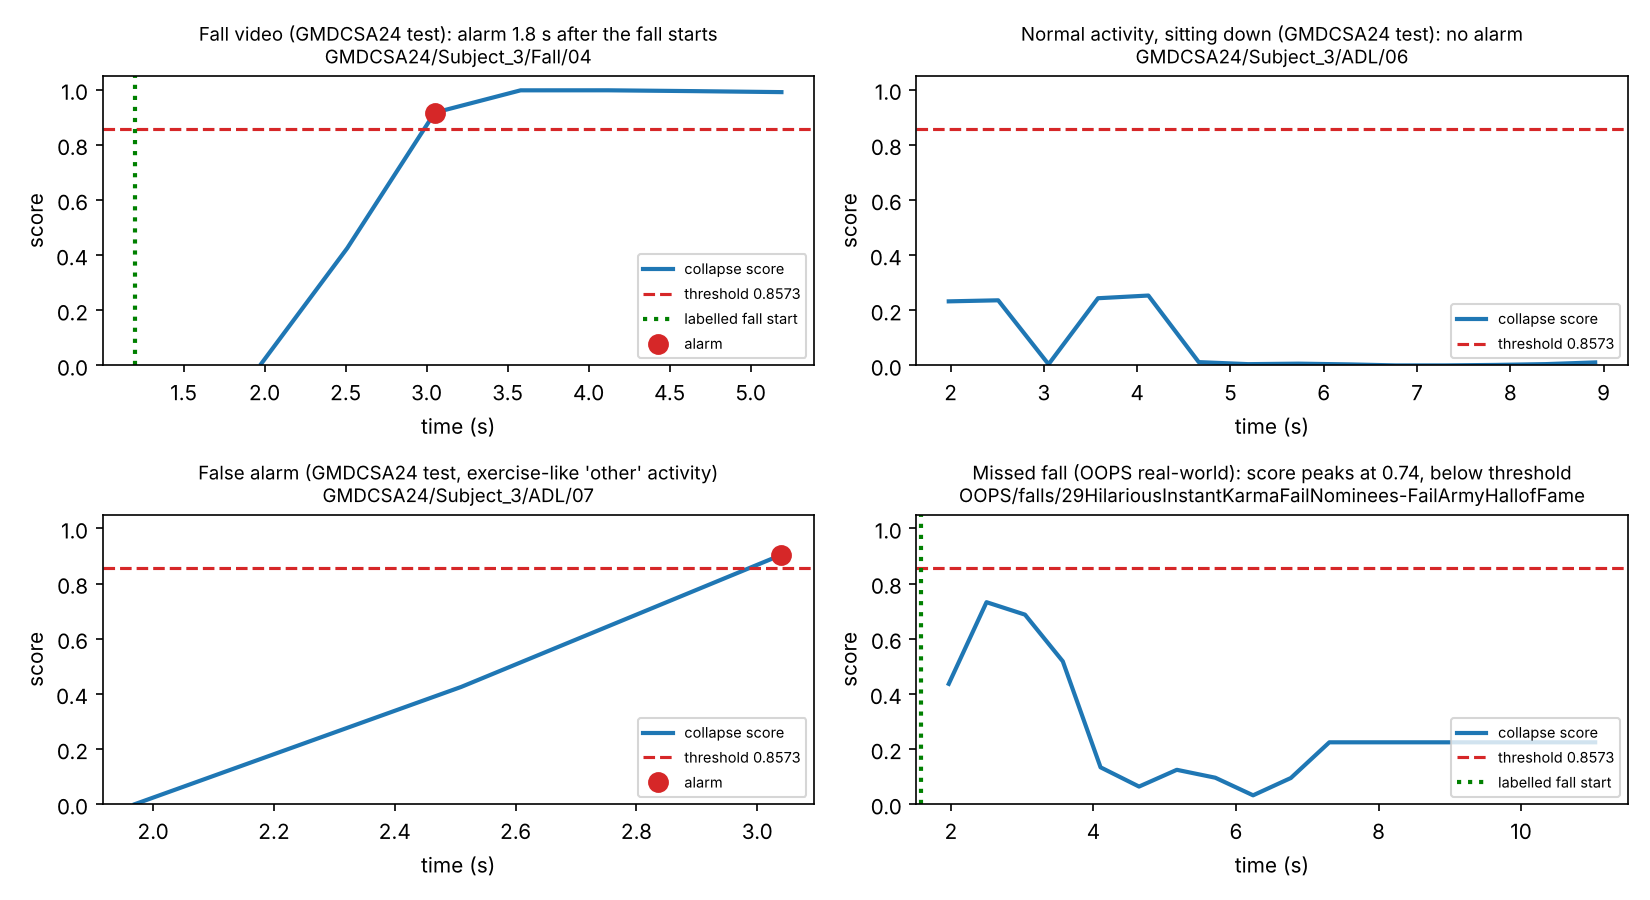
\includegraphics[width=\textwidth]{score_traces.png}
\caption{Collapse score of the submitted engine over time (one point per 0.5\,s stride; the first window needs 2\,s of history). Top left: a fall is caught 1.8\,s after the labelled start. Top right: sitting down stays far below the threshold. Bottom left: a false alarm on an exercise-like activity. Bottom right: a real-world OOPS fall whose score peaks at 0.74 and is missed.}\label{fig:traces}
\end{figure}

\subsection{Speed and deployment (\code{src/speed\_test.py}, \code{app/})}
29.6 frames/s on a Tesla T4 (15 are needed for real time; \code{results/speed.md}); the GRU takes 0.1\,ms
per frame. On a laptop CPU we measured about 2--3 frames/s with PyTorch and 10--13 frames/s with an optional
OpenVINO conversion that only the interactive programs use. \code{app/live\_fall.py} runs the same engine live from a webcam, a phone camera or an
RTSP stream, for any number of people.

\section{Training and validation curves}
Figure~\ref{fig:curves} shows, per epoch, the class-weighted cross-entropy and the window macro-F1 on a fixed
sample of training windows (without augmentation) and on the validation windows, for the final GRU and the two
comparison GRUs. The curves were obtained by re-running \code{src/train\_gru.py} with identical data, settings
and seed in order to record every epoch (\code{notebooks/07\_training\_curves.ipynb}); the orange star is the
submitted \code{gru\_hard.pt} (kept at epoch 16) measured on the same validation windows, and it lies on the
re-run's validation curve (loss 0.363 vs 0.378, macro-F1 0.864 vs 0.862 at epoch 16), so the figure describes
the submitted training. GPU training is not bit-identical, which is why the re-run's best epoch (8, 0.865)
differs slightly from the original's (16, 0.864). The pipeline now writes these curves on every training run.

\begin{figure}[H]\centering
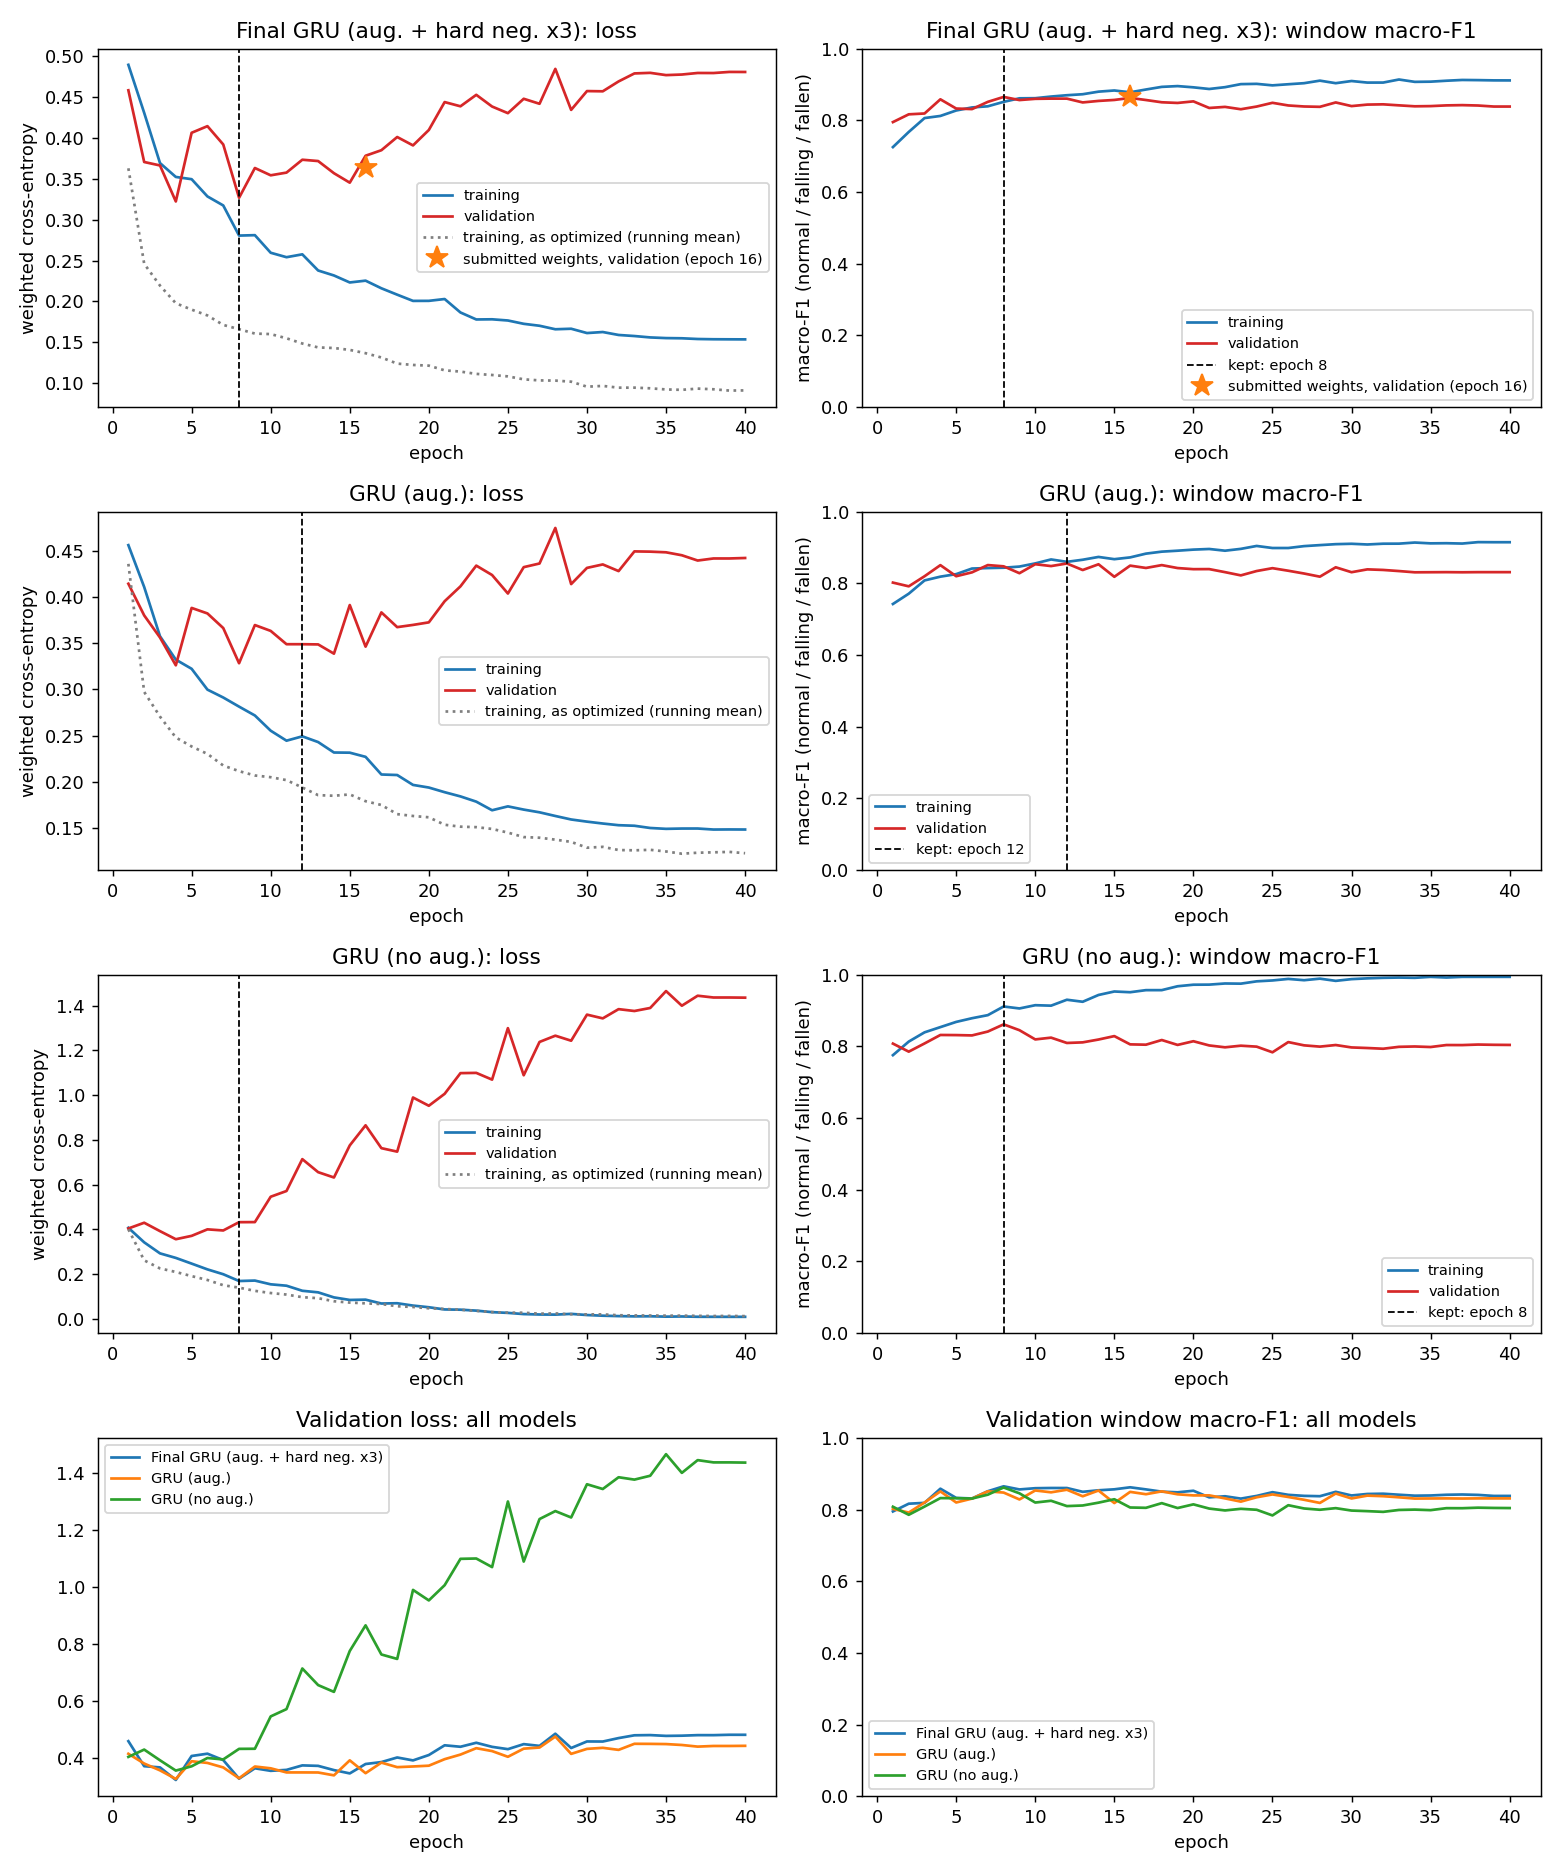
\includegraphics[width=0.96\textwidth]{training_curves.png}
\caption{Training (blue) and validation (red) loss and window macro-F1 per epoch; dotted: the loss actually optimised (with augmentation and hard-negative weights); dashed: the epoch kept; star: the submitted weights. Bottom row: validation curves of all three models.}\label{fig:curves}
\end{figure}

\begin{table}[H]\centering\footnotesize
\begin{tabular}{@{}lcccc@{}}\toprule
\textbf{Model} & \textbf{Best epoch} & \textbf{Val macro-F1} & \textbf{Train / val loss} & \textbf{Train / val macro-F1}\\ \midrule
Final GRU (augmentation + hard negatives $\times 3$) & 8 & 0.865 & 0.281 / 0.327 & 0.851 / 0.865\\
GRU, augmentation only & 12 & 0.855 & 0.249 / 0.349 & 0.860 / 0.855\\
GRU, no augmentation & 8 & 0.862 & 0.168 / 0.431 & 0.912 / 0.862\\
Submitted weights (\code{gru\_hard.pt}) & 16 & 0.864 & -- / 0.363 & -- / 0.864\\
\bottomrule\end{tabular}
\caption{Learning-curve summary (\code{results/training\_curves.md}).}
\end{table}

\textbf{Reading the curves.} Without augmentation the model overfits: training loss falls to almost zero and
training macro-F1 to 1.0 while the validation loss climbs from about epoch 5 (0.36 $\rightarrow$ 1.44) and
validation macro-F1 drifts down to 0.80. With augmentation the gap stays small (training loss 0.15--0.28
against validation 0.33--0.48) and validation macro-F1 stays on a plateau of 0.84--0.87 for the whole run.
Validation macro-F1 peaks early (epochs 8--16) and the validation loss rises slowly afterwards, which is why
the best-validation epoch is kept rather than the last one. Hard negatives change the window-level curves
little; their effect is on video-level false alarms, which is why the final choice was made on video-level
validation F1 (Section 4.6).

\section{Results}
\subsection{Submitted system}
\begin{table}[H]\centering\footnotesize
\begin{tabular}{@{}lrrrrrrr@{}}\toprule
\textbf{Split} & \textbf{Videos} & \textbf{F1} & \textbf{Prec.} & \textbf{Recall} & \textbf{False alarms} & \textbf{Missed falls} & \textbf{Median delay}\\ \midrule
validation (reference) & 76 & 0.965 & 0.932 & 1.000 & 3 & 0 & 1.6\,s\\
test GMDCSA24 S3--4 & 80 & 0.875 & 0.833 & 0.921 & 7 & 3 & 1.9\,s\\
test staged (Le2i, CAUCAFall) & 57 & 0.968 & 0.968 & 0.968 & 1 & 1 & 1.5\,s\\
test OOPS (real world) & 818 & 0.855 & 0.958 & 0.772 & 25 & 169 & 1.1\,s\\
own recordings & 20 & 0.857 & 1.000 & 0.750 & 0 & 5 & 1.0\,s\\
\bottomrule\end{tabular}
\caption{The submitted frame-by-frame system (\code{infer.py} engine, threshold 0.8573 chosen on validation, each test set run once; \code{results/causal\_eval.md}).}\label{tab:final}
\end{table}

\begin{figure}[H]\centering
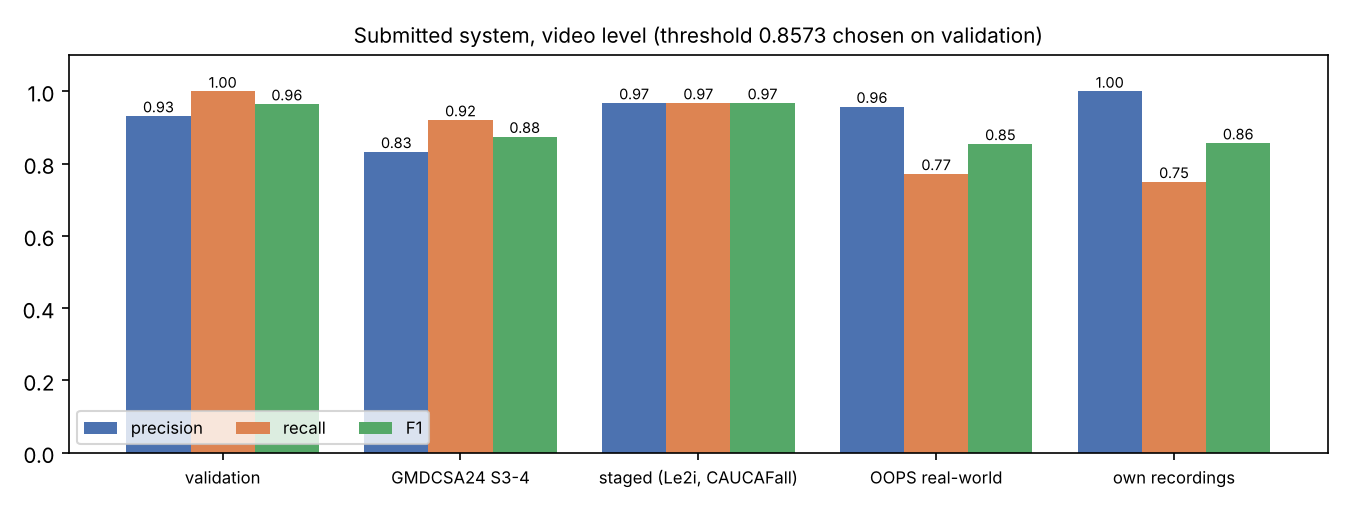
\includegraphics[width=0.9\textwidth]{results_bars.png}
\caption{Precision, recall and F1 of the submitted system per split (Table~\ref{tab:final}).}
\end{figure}

Own recordings: the night fall is caught; the misses are two far-away people, one fall inside a group of three
(the faller's track splits at the fall), one fall from sitting (score 0.63) and one at 0.71. Other
measurements: alarm box on the right person in 92\,\% of checked alarms; estimated onset within 0.3--0.5\,s of
the label; alarm 1.0--1.9\,s after the fall starts.

\subsection{Model comparison}
\begin{figure}[H]\centering
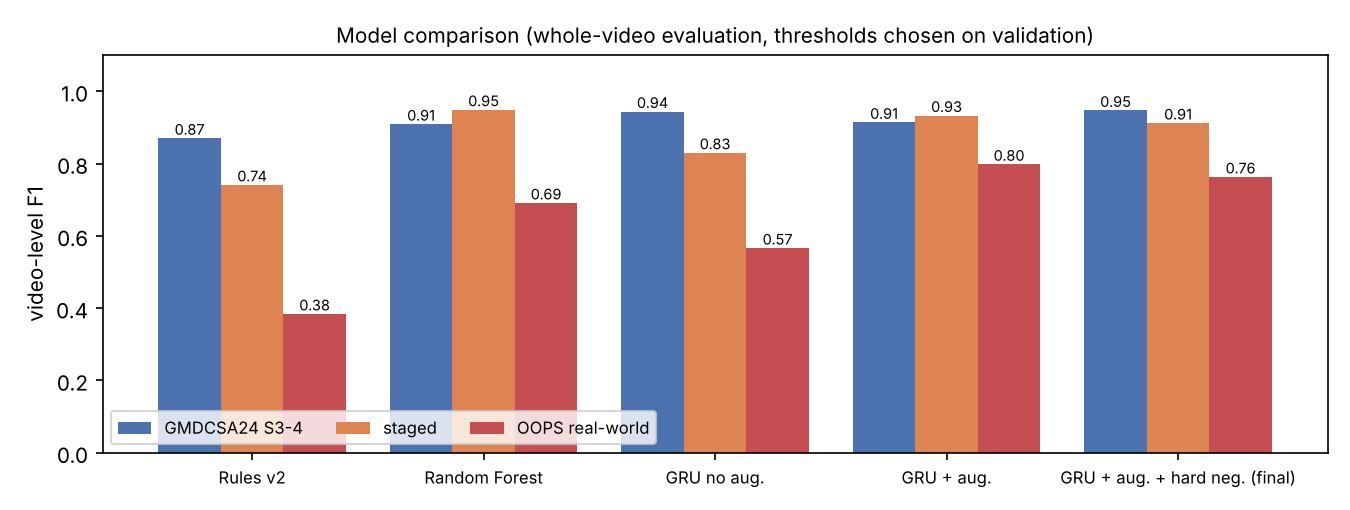
\includegraphics[width=0.9\textwidth]{model_comparison.png}
\caption{Video-level F1 of every approach on the three public test sets (whole-video evaluation, thresholds chosen on validation; \code{results/*.md}).}\label{fig:models}
\end{figure}
Augmentation is what makes the model work on real-world video (OOPS F1 0.57 $\rightarrow$ 0.80); hard
negatives trade a little OOPS recall for fewer false alarms on the staged sets and gave the best validation F1,
which is why that model was chosen --- the choice was made on validation, not on the test numbers in
Figure~\ref{fig:models}.

\section{Failure cases}
\begin{table}[H]\centering\small
\begin{tabularx}{\textwidth}{@{}>{\raggedright\arraybackslash}p{4.2cm}X@{}}\toprule
\textbf{Failure} & \textbf{Cause} \\ \midrule
Very small / far person & YOLO loses the person exactly when they fall; 9 of the 12 worst OOPS misses had the person detected in only 6--21\,\% of frames (own videos 002, 009). \\
Moving or shaking camera (OOPS) & Image motion is mistaken for body motion. \\
Very fast or blurred fall; person leaving the frame & Too few clear frames in the 2-s window. \\
Fall inside a group (own video 011) & The tracker gives the faller a new ID; the window is split. \\
Fall from sitting (own video 013) & Score 0.63, below the threshold, in the frame-by-frame system (it was caught when the whole clip was visible): causal operation costs a little recall here. \\
False alarms & Lying down on purpose (2 of 6 analysed), push-ups / exercise (1 of 6); more people in view means more chances of a false alarm. \\
Label problems & E.g.\ a GMDCSA24 fall labelled ``lie down''; 77 OOPS clips without a fall label. \\
\bottomrule\end{tabularx}
\caption{Failure cases (\code{results/error\_analysis.md}, own-video diagnosis, hard validation set).}
\end{table}
Ideas tested and not kept: image brightening at night, zoom re-check for small people, input 1280, low-confidence
tracking, fall-aware track joining, a higher threshold from the hard validation set, decision lag $>0$, model
averaging (all with numbers in \code{results/summary.md}).

\section{Reproducibility}
\begin{itemize}
\item \textbf{Environment:} Python 3.13, PyTorch 2.11.0 (+CUDA 13.0 on Kaggle, CPU build on a laptop),
Ultralytics 8.4.212; every version is pinned in \code{requirements.txt} and recorded in
\code{results/env\_kaggle.txt}. Inference runs on CPU or GPU (\code{--device cpu | cuda | cuda:N | N}, with CPU
fallback).
\item \textbf{One command:} \code{python run\_pipeline.py --omnifall-root DATA/omnifall --gmd-root DATA/GMDCSA24
--work work --all-models --device cuda:0} runs pose caching, features, windows, training (with curves), model
choice and the final evaluation; a re-run re-chooses the threshold on validation and writes it to
\code{config.yaml}. The same runs on Kaggle in \code{kaggle/project\_kaggle.ipynb} or in stages
(\code{notebooks/03--05}).
\item \textbf{Tests:} \code{python -m pytest tests} (14 tests: syntax, config, device handling, model
forward, a small training run with checkpoints and curves, metrics, and \code{infer.py} on the two example clips).
\item \textbf{Verification example:} \code{examples/videos} (two GMDCSA24 clips, MIT licence) with the
expected output files; \code{python make\_submission.py --verify} re-runs it from an unzipped copy of the project.
\item \textbf{Documentation:} \code{README.md}, \code{APPROACHES\_AND\_EXPERIMENTS.md}, \code{METHODOLOGY.md},
\code{REPRODUCIBILITY.md}, \code{KAGGLE\_INSTRUCTIONS.md}, \code{docs/DATA.md}, \code{docs/PROJECT.md}.
\end{itemize}

\section{Individual contributions}
\begin{table}[H]\centering\small
\begin{tabularx}{\textwidth}{@{}lX@{}}\toprule
\textbf{Member} & \textbf{Contributions}\\ \midrule
Member 1 & Data and evaluation: labelled 18 of the team's own videos (fall type, start time, lighting, distance, number of people) in the label sheet used by the evaluation scripts; manual localization study (36 alarm frames checked by eye), which gives the 92\,\% figure; watched and classified the missed falls and false alarms for the error analysis.\\[2pt]
Member 2 & Design and implementation of the system: OmniFall-based splits, pose caching with YOLO11m-pose and ByteTrack, the 92 skeleton features and 2-s windows, the GRU models (augmentation, hard negatives) and the Random Forest baseline, model and threshold selection on validation, the frame-by-frame inference engine and \code{infer.py}, the evaluation scripts, the night / far-away robustness experiments, the Kaggle pipeline notebooks, documentation and the submission package; repository owner.\\[2pt]
Member 3 & Test data: planned and recorded the 20 own test videos (day and night, near and far, one to nine people; falls from standing, walking, sitting and jumping) following the recording plan, kept in a private dataset; ran the own-video checker and the own-video evaluations and reported their results.\\
\bottomrule\end{tabularx}
\end{table}

\begin{thebibliography}{9}\small
\bibitem{yolo11} G.~Jocher and J.~Qiu, \emph{Ultralytics YOLO11}, 2024. \url{https://github.com/ultralytics/ultralytics}
\bibitem{bytetrack} Y.~Zhang et al., ``ByteTrack: Multi-Object Tracking by Associating Every Detection Box,'' \emph{ECCV}, 2022.
\bibitem{omnifall} OmniFall: unified labels and cross-subject splits for fall-detection datasets, Hugging Face \code{simplexsigil2/omnifall}.
\bibitem{gmdcsa} GMDCSA24: a dataset for human fall detection in videos (GitHub release, MIT licence).
\bibitem{le2i} I.~Charfi et al., ``Optimized spatio-temporal descriptors for real-time fall detection: comparison of SVM and Adaboost-based classification,'' \emph{J.\ Electronic Imaging}, 2013 (Le2i fall dataset).
\bibitem{caucafall} J.~Eraso et al., ``CAUCAFall: a dataset for fall detection,'' Mendeley Data, 2022.
\bibitem{mcfd} E.~Auvinet et al., ``Multiple cameras fall dataset,'' Technical report 1350, DIRO, Université de Montréal, 2010.
\bibitem{oops} D.~Epstein, B.~Chen and C.~Vondrick, ``Oops! Predicting Unintentional Action in Video,'' \emph{CVPR}, 2020.
\bibitem{gru} K.~Cho et al., ``Learning Phrase Representations using RNN Encoder--Decoder for Statistical Machine Translation,'' \emph{EMNLP}, 2014.
\end{thebibliography}

\end{document}
